\section{System Design\label{sec:systemDesign}}
In this section, we provide an overview of visual encoding for blazar data and the visual exploration framework of TimeTubesX.

\begin{figure}[tb]
    \begin{minipage}{0.34\linewidth}
        \centering
        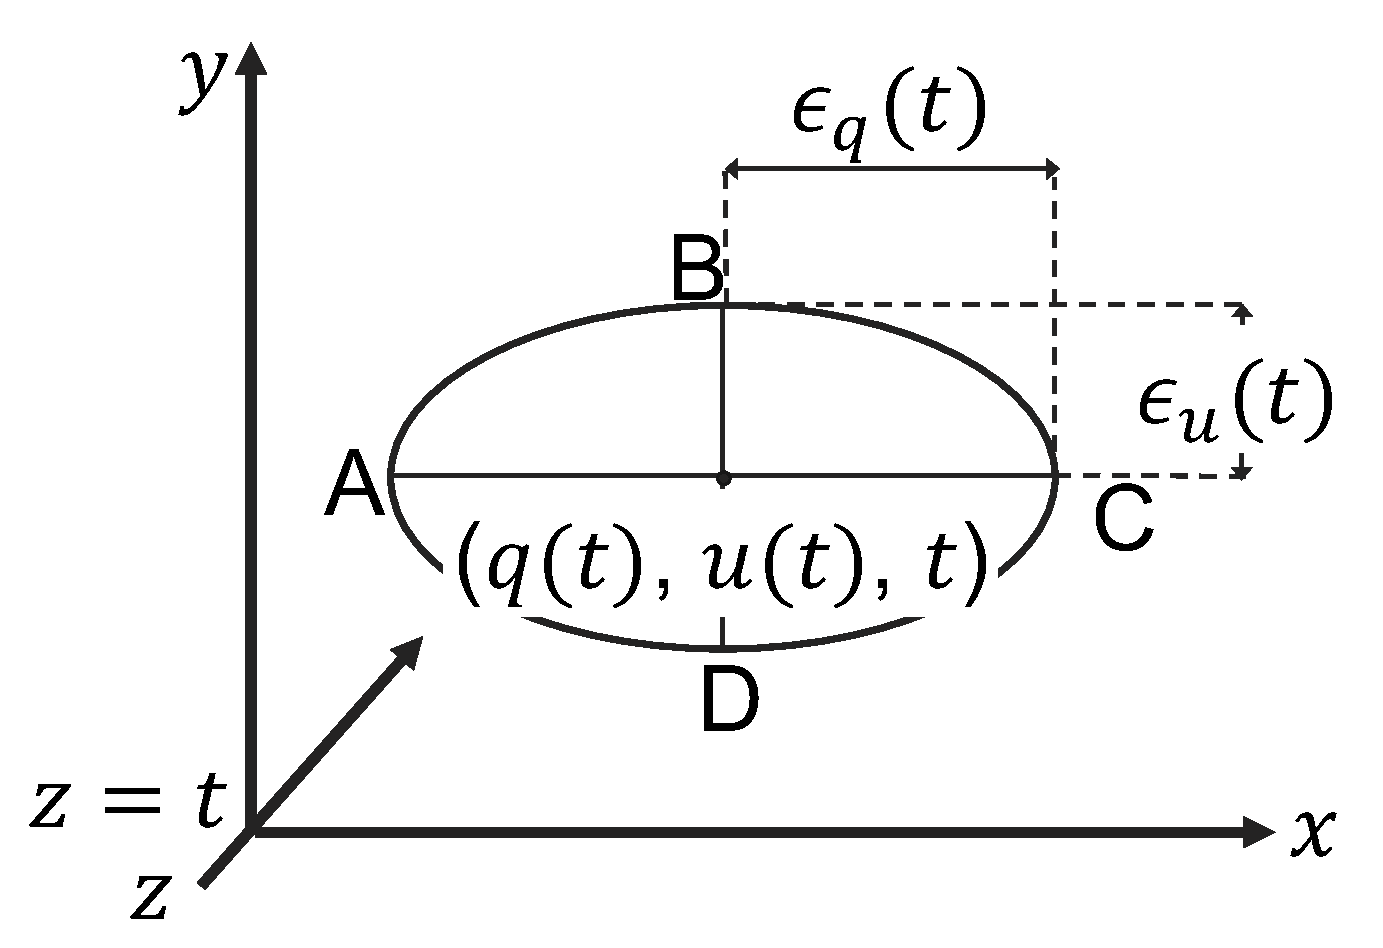
\includegraphics[width=.99\linewidth]{vgtc_journal_latex/figures/howtoplot.pdf}
    \end{minipage}
    \begin{minipage}{0.26\linewidth}
        \centering
        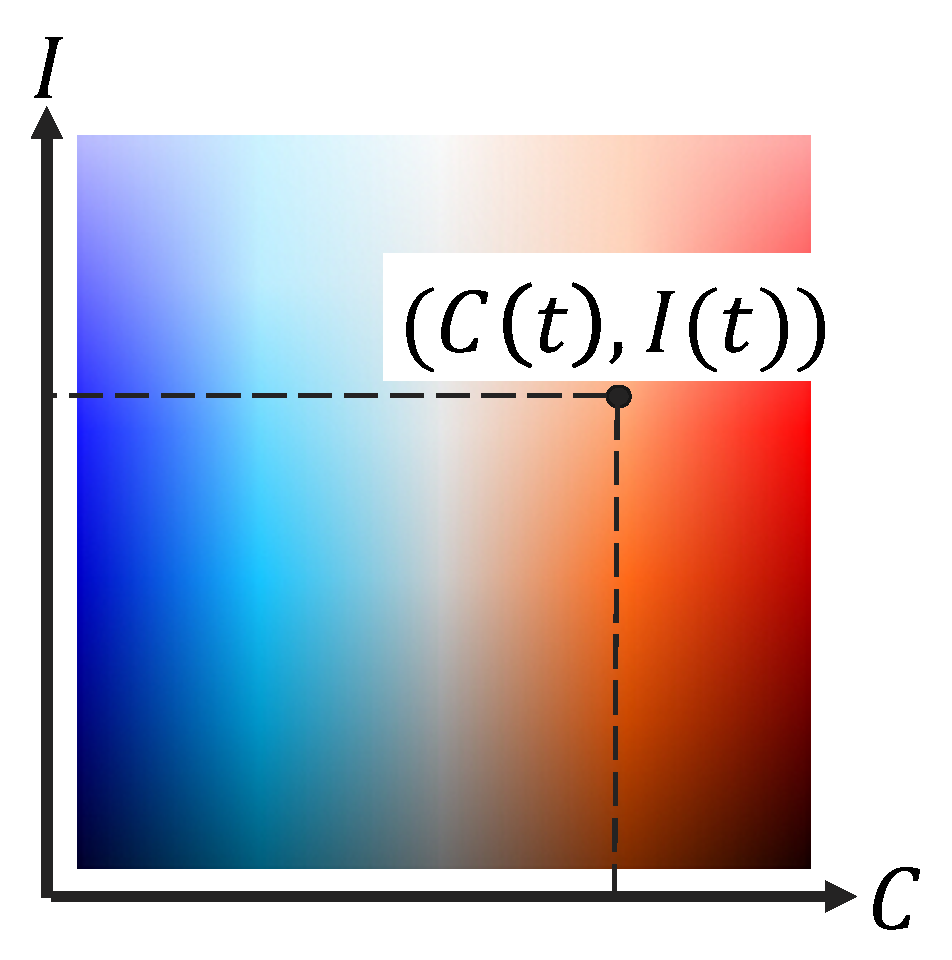
\includegraphics[width=.99\linewidth]{vgtc_journal_latex/figures/colormap.pdf}
    \end{minipage}
    \begin{minipage}{0.36\linewidth}
        \centering
        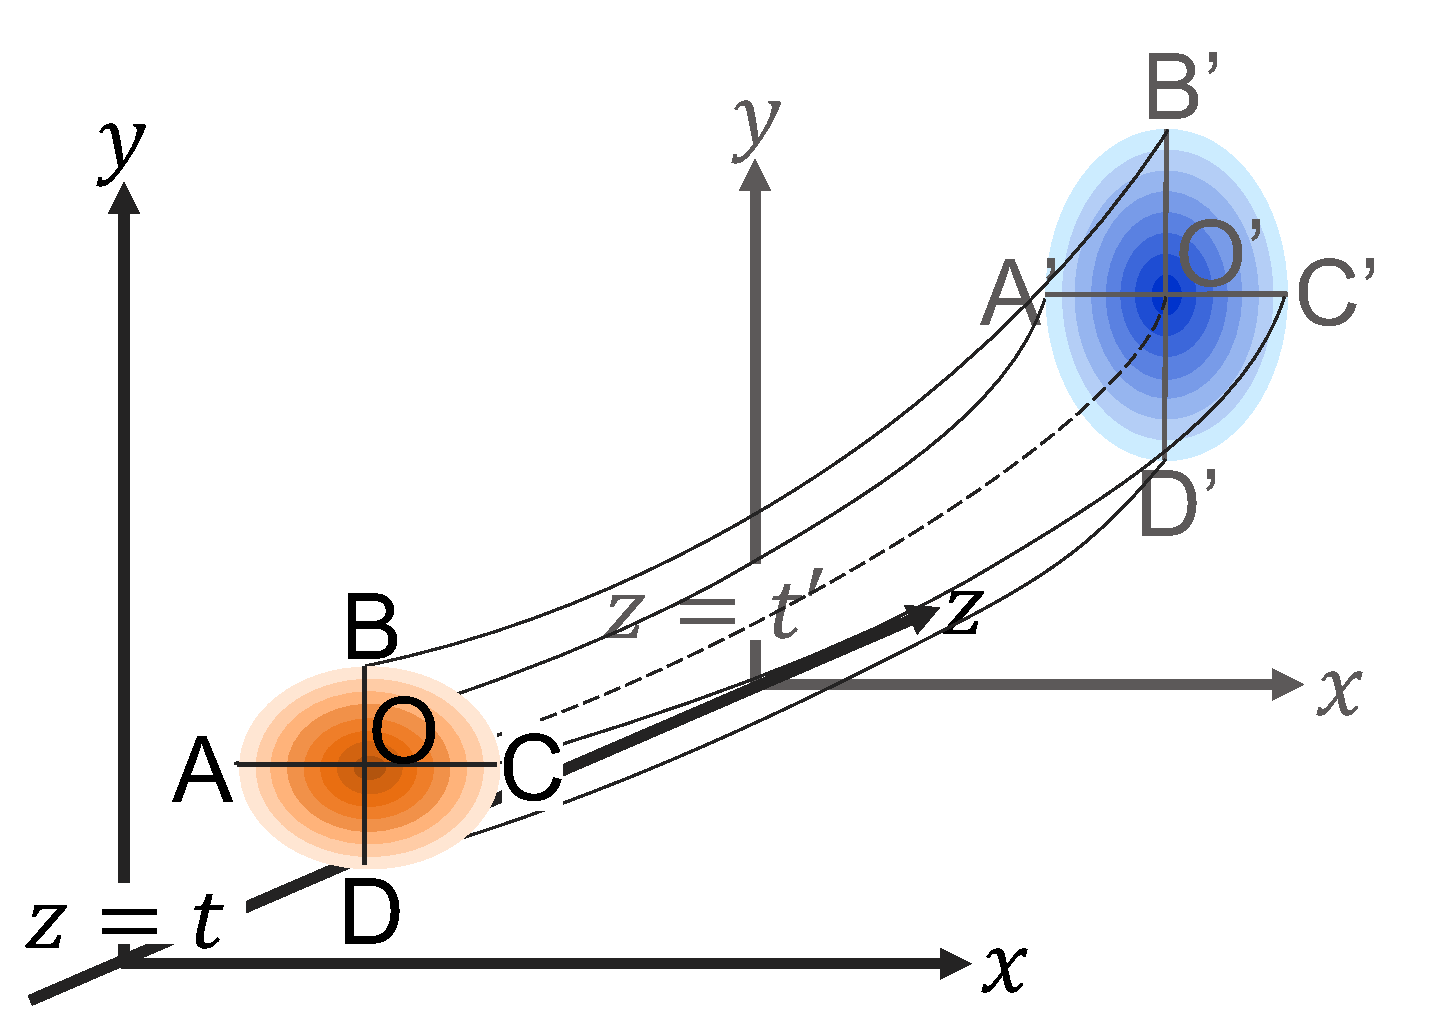
\includegraphics[width=.99\linewidth]{vgtc_journal_latex/figures/howtotube.pdf}
    \end{minipage}
    \begin{minipage}{0.34\linewidth}
        \centering
        \footnotesize{\sf (a)}
        \end{minipage}
    \begin{minipage}{0.26\linewidth}
        \centering
        \footnotesize{\sf (b)}
    \end{minipage}
    \begin{minipage}{0.36\linewidth}
        \centering
        \footnotesize{\sf (c)}
    \end{minipage}
    \caption{Spatial mapping in the TimeTubes view. 
    (a)~Observation values of polarization decide the position and shape of an ellipse;
    (b)~observation values of intensity and color colorize the ellipse with reference to a colormap; and
    (c)~the neighboring ellipses are smoothly connected in chronological order to yield a tube shape.}
    \label{fig:howtoplot}
\end{figure}
\subsection{Visual Encoding for Blazar Data}\label{sec:VisualEncoding}
\begin{figure*}
    \centering
    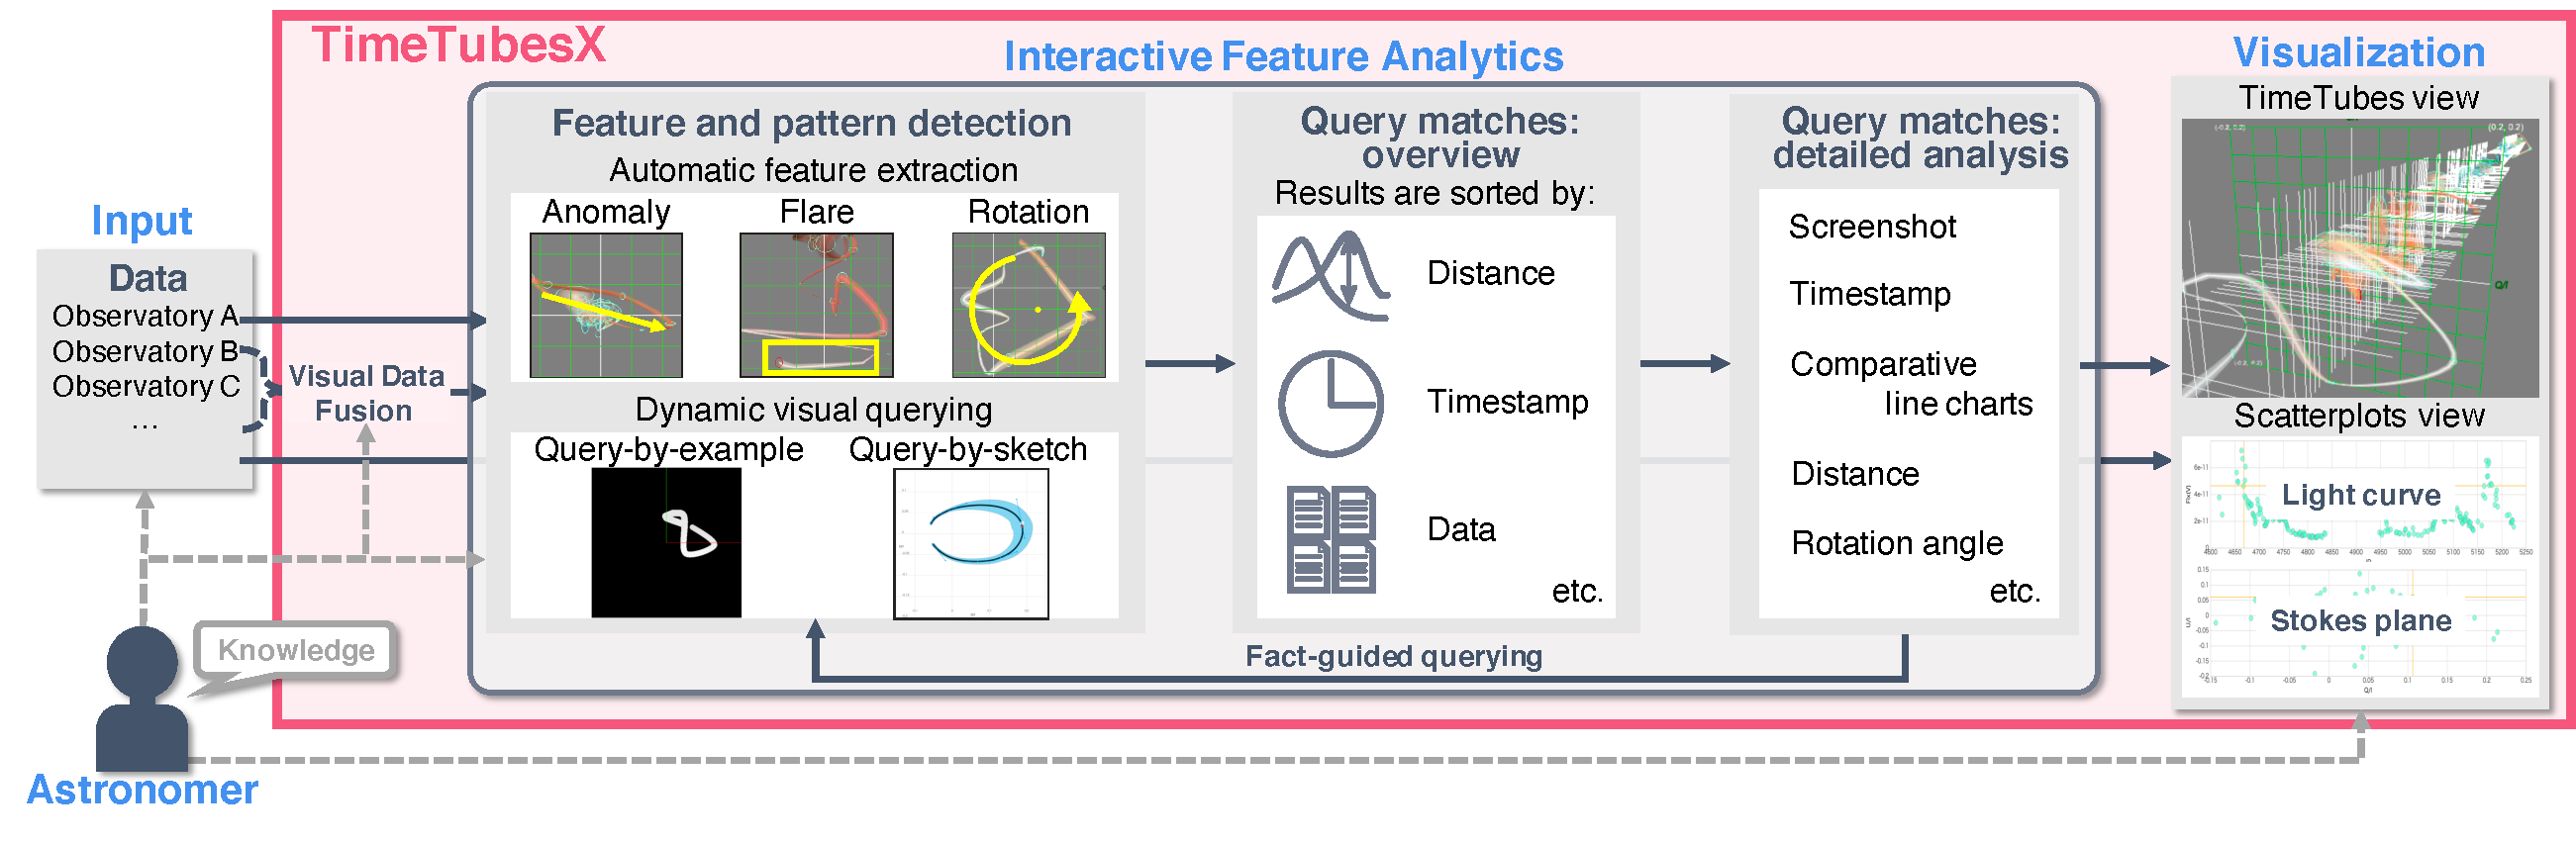
\includegraphics[width=.99\linewidth]{vgtc_journal_latex/figures/workflowGray.pdf}
    \caption{The visual exploration framework of TimeTubesX. Users can load multiple datasets into a single exploration session through visual data fusion. (A)~Users specify a query to extract features of interest; (B)~query results are sorted by relevance; (C)~individual results can be analyzed in high detail and compared to each other; (D)~an extraction result can be re-used as an input for a new visual query; and (E)~users can visually explore the results in the TimeTubes and scatterplots views.}
    \label{fig:framework}
\end{figure*}
Astronomers have used three animated scatterplots with error bars to visualize their multi-dimensional, time-dependent observations (see the accompanying video): one for time variation of $I$, termed \textit{light curve}, another for the Stokes plane, and a third for the correlation between $I$ and $C$.
During the animation, individual observations are highlighted in red in order of observation.

Instead of animating multiple 2D scatterplots,
TimeTubesX expresses blazar observations as a single 3D volumetric tube. 
In the following part, we give an overview of the \emph{TimeTubes view}, which was originally proposed in our previous work~\cite{Fujishiro2018}.
The TimeTubes view allows users to see correlations and variations of variables over time at a glance, as illustrated in Fig.~\ref{fig:framework}~(E).
In the current version, users need to import .csv files with column names from their local environment into TimeTubesX.
We use a left-handed coordinate system to assign $q$ and $u$ to the $x$ and $y$ axes, respectively, and time $t$ to the $z$ axis.
We encode the polarization parameters ($q$, $u$, $\epsilon_q$, $\epsilon_u$) at each timestamp $t$ as an ellipse centered at the point $(x, y, z) = (q(t), u(t), t)$ with a width of $2\epsilon_q(t)$ and a height of $2\epsilon_u(t)$, as depicted in Fig.~\ref{fig:howtoplot}~(a). 
Therefore, the $x$--$y$ location of an ellipse indicates the polarization at a certain time stamp, while the size of the ellipse indicates the uncertainty of the measurement.
To properly render a 3D tube, we set the value range of the Stokes plane in the TimeTubes view with reference to the standard deviations of $q$ and $u$ in the datasets. 
In the current TimeTubes view, we empirically map a single day to a single voxel along the $z$ axis.
We colorize the ellipses according to $I(t)$ and $C(t)$ based on a user-defined 2D colormap (Fig.~\ref{fig:howtoplot}~(b)). 
The TimeTubes view connects neighboring ellipses in chronological order, using centripetal Catmull-Rom splines to form a 3D volumetric tube (Fig.~\ref{fig:howtoplot}~(c)). 
To further reflect the reliability of the observations, the TimeTubes view offers an adjustable opacity transfer function.
Multiple concentric tubes with different transparencies (i.e., higher opacities for inner tubes) compose a single tube that allows users to intuitively perceive the uncertainties of observations.
Specifically, a time interval with small errors looks like an opaque tube, whereas a time interval with large errors looks more semi-transparent and fuzzy.

Compared with the initial animated scatterplots,
the TimeTubes view provides more uncertainty-aware visual encoding for the analysis of blazar behaviors (\textbf{T1}).
Astronomers do not need to scrutinize multiple plots to understand correlations between variables
or move sliders back and forth 
to track time variations.


\subsection{Visual Exploration Framework\label{sec:approach}}
The design of TimeTubesX supports the visualization tasks outlined in Section~\ref{sec:domainGoalsandTasks}.
Fig.~\ref{fig:framework} illustrates our visual exploration framework.
%
The user workflow starts with visual data fusion~\cite{Fujishiro2018} to create a unified dataset for all subsequent analysis steps (\textbf{T2}).
For initial feature and pattern detection (A), users can either rely on automatic feature extraction methods for well-known blazar behaviors (\textbf{T3}) or define their own visual queries for a ROI/SOI (\textbf{T4}, \textbf{T5}).
The system ranks the results of the feature and pattern detection stage and shows the ranked matches (B).
Users can sort the results to, for instance, focus on time intervals that have the largest rotation or are the most similar to the input pattern.
The detailed analysis (C) helps users understand the behavior at the extracted time intervals and classify the results. 
To support iterative refinement of queries, users can build a follow-up query based on the result of a query (D). It allows users to find time intervals similar to the result (\textbf{T4}).
We call this \textit{fact-guided querying}, as it enables users to refine extraction results guided by previously detected features.
To analyze extracted time intervals in more detail, users can employ
the uncertainty-aware TimeTubes view (\textbf{T1}) as well as multiple linked scatterplots views (E).

\textsf{Interactive feature analysis interface.\ } 
Fig.~\ref{fig:UIFeatureExtraction} shows our feature and pattern detection user interface. 
The query specification panel (A) allows users 
to build a query with simple interactions either by selecting what to extract, picking a part of data as an input, or sketching time variation patterns.
After running a similarity search, 
TimeTubesX ranks and filters extraction results according to the parameters in panel (B),
and then it displays all relevant (i.e., non-filtered) extraction results as a collection of thumbnails in panel (E).
The distance distribution histogram in panel (B) helps users to further filter the number of results.
The timeline in panel (C) gives an overview of the temporal distribution of the results.
Users are able to recognize groups of results sharing identical data samples and temporal distribution features.
When selecting an individual thumbnail, TimeTubesX shows a detailed information on the corresponding result in panel (D), including exact timestamps and the distance between the query and the result.
To re-utilize the query, compare multiple query results, and share the query and their results with other users, 
TimeTubesX allows users to export and import queries and their results in the form of JSON files (a custom format for TimeTubesX).
When importing previous query results,
panel (F) shows a summary of the query used in the previous process and panel (C) shows another timeline for the imported query results.

Fig.~\ref{fig:querySpecificationPanel} shows the query specification panels for each mode of the feature and pattern detection.


To better demonstrate our feature and pattern detection methods, we will use a synthetic dataset (see Fig.~\ref{fig:synthesisData}) as a running example in Sections~\ref{sec:automaticExtraction} and \ref{sec:visualQuery}.
It contains four large peaks in $I$, as highlighted by orange diamonds in (a), three small red circular patterns on the Stokes plane in (b), three large green rotations , and three narrow/rough-edged blue patterns.
